%%%%%%%% ICML 2021 EXAMPLE LATEX SUBMISSION FILE %%%%%%%%%%%%%%%%%

\documentclass{article}

% Recommended, but optional, packages for figures and better typesetting:
\usepackage{microtype}
\usepackage{graphicx}
\usepackage{subfigure}
\usepackage{booktabs} % for professional tables

% hyperref makes hyperlinks in the resulting PDF.
% If your build breaks (sometimes temporarily if a hyperlink spans a page)
% please comment out the following usepackage line and replace
% \usepackage{icml2021} with \usepackage[nohyperref]{icml2021} above.
\usepackage{hyperref}

% Attempt to make hyperref and algorithmic work together better:
\newcommand{\theHalgorithm}{\arabic{algorithm}}

% Use the following line for the initial blind version submitted for review:
\usepackage{icml2021}

% If accepted, instead use the following line for the camera-ready submission:
%\usepackage[accepted]{icml2021}

% The \icmltitle you define below is probably too long as a header.
% Therefore, a short form for the running title is supplied here:
\icmltitlerunning{Nonparametric tensor completion}
\usepackage{mathrsfs}
\usepackage{wrapfig}
\usepackage{multirow}
\usepackage{graphicx}
%\usepackage[utf8]{inputenc} % allow utf-8 input
%\usepackage[T1]{fontenc}    % use 8-bit T1 fonts
\usepackage{hyperref}       % hyperlinks
\usepackage{url}            % simple URL typesetting
%\usepackage{booktabs}       % professional-quality tables
\usepackage{amsmath,amssymb}
\usepackage{amsthm}    % blackboard math symbols
%\usepackage{nicefrac}       % compact symbols for 1/2, etc.
%\usepackage{microtype}      % microtypography
\usepackage{bm}
%\usepackage{subfig}
%\usepackage[english]{babel}
%\usepackage{algorithm}
%\usepackage{appendix}
\usepackage{mathtools}
\mathtoolsset{showonlyrefs}
\usepackage{enumitem}
\theoremstyle{plain}
\newtheorem{thm}{Theorem}[section]
\newtheorem{lem}{Lemma}
\newtheorem{prop}{Proposition}
\newtheorem{pro}{Property}


\theoremstyle{definition}
\newtheorem{defn}{Definition}
\newtheorem{assumption}{Assumption}
\newtheorem{cor}{Corollary}
\newtheorem{example}{Example}
\newtheorem{rmk}{Remark}

\usepackage{dsfont}
%\usepackage{algpseudocode,algorithm}
%\algnewcommand\algorithmicinput{\textbf{Input:}}
%\algnewcommand\algorithmicoutput{\textbf{Output:}}
%\algnewcommand\INPUT{\item[\algorithmicinput]}
%\algnewcommand\OUTPUT{\item[\algorithmicoutput]}
%\DeclareMathOperator*{\minimize}{minimize}

\usepackage{xr}



\newcommand*{\KeepStyleUnderBrace}[1]{%f
  \mathop{%
    \mathchoice
    {\underbrace{\displaystyle#1}}%
    {\underbrace{\textstyle#1}}%
    {\underbrace{\scriptstyle#1}}%
    {\underbrace{\scriptscriptstyle#1}}%
  }\limits
}
\usepackage{makecell}
\input macros.tex

\usepackage{amssymb}
\usepackage{pifont}
\newcommand{\cmark}{\ding{51}}%
\newcommand{\xmark}{\ding{55}}%
\def\sign{\textup{sgn}}
\def\srank{\textup{srank}}
\def\rank{\textup{rank}}
\def\caliP{\mathscr{P}_{\textup{sgn}}}
\def\risk{\textup{Risk}}

\begin{document}

\twocolumn[
\icmltitle{Beyond the Signs: Nonparametric Tensor Completion via Sign Series}

\icmlsetsymbol{equal}{*}

\begin{icmlauthorlist}
\icmlauthor{Chanwoo Lee}{wisc}
\icmlauthor{Miaoyan Wang}{wisc}
\end{icmlauthorlist}

\icmlaffiliation{wisc}{Department of Statistics, University of Wisconsin -- Madison}


\icmlcorrespondingauthor{Miaoyan Wang}{miaoyan.wang@wisc.edu}


% You may provide any keywords that you
% find helpful for describing your paper; these are used to populate
% the "keywords" metadata in the PDF but will not be shown in the document
\icmlkeywords{Higher-order tensors, completion, sliced inverse regression, probability estimation}

\vskip 0.3in
]

% this must go after the closing bracket ] following \twocolumn[ ...

% This command actually creates the footnote in the first column
% listing the affiliations and the copyright notice.
% The command takes one argument, which is text to display at the start of the footnote.
% The \icmlEqualContribution command is standard text for equal contribution.
% Remove it (just {}) if you do not need this facility.

\printAffiliationsAndNotice{}  % leave blank if no need to mention equal contribution


\begin{abstract}
We consider the problem of tensor estimation from noisy observations with missing entries. A nonparametric approach to tensor completion is developed based on a new model which we coin as ``sign representable tensors.'' The model represents a continuous-valued signal tensor using a series of sign tensors with low sign-ranks. Unlike earlier methods, the sign series representation effectively addresses both low- and high-rank signal tensors, while encompassing many existing tensor models---including CP models, Tucker models, single index models, certain hypergraphon models---as special cases. We show that the sign tensor series are theoretically characterized, and computationally solvable, by classification tasks with carefully-specified weights. The excess risk rate, estimation error bound, and sample complexity are established. The results uncover the joint contribution of statistical bias-variance errors and discretization errors. Numerical results demonstrate the robustness of our proposal over previous tensor methods.
\end{abstract}

\section{Introduction}\label{Intro}

Advantages:
(1) exactly recovers the signal tensor under a wide range of low- and high-rank tensor models; 
(2) brings the nonparametric advantages of flexibility into tensor estimation and completion; 
(3) achieves computational efficiency by leveraging classification and divide-and-conquer algorithms.

\section{Preliminaries}
We use the shorthand $[n]$ to denote the $n$-set $\{1,\ldots,n\}$ for $n\in\mathbb{N}_{+}$. We use $\otimes$ to denote the outer product of vectors, $\vnormSize{}{\mx}$ to denote the vector $2$-norm, and $\mathbf{S}^{d-1}=\{\mx\in\mathbb{R}\colon \vnormSize{}{\mx}=1\}$ to denote the $(d-1)$-dimensional unit sphere. Let $\tY\in\mathbb{R}^{d_1\times \cdots \times d_K}$ denote an order-$K$ $(d_1,\ldots,d_k)$-dimensional tensor, and $\tY(\omega)\in\mathbb{R}$ denote the tensor entry indexed by $\omega \in[d_1]\times \cdots \times [d_K]$. The Frobenius norm of $\tY$ is defined as $\FnormSize{}{\tY}=\sqrt{\sum_{\omega}\tY^2(\omega)}$. Unlike matrices, various notions of decomposition have been developed for tensors of order $K\geq 3$. The Canonical Polyadic (CP) tensor decomposition~\cite{hitchcock1927expression} for a tensor $\Theta\in\mathbb{R}^{d_1\times \cdots \times d_K}$ is defined as
\begin{equation}\label{eq:CP}
\Theta=\sum_{s=1}^r\lambda_s \ma^{(1)}_s\otimes\cdots\otimes \ma^{(K)}_s,
\end{equation}
where $\lambda_1\geq \cdots \geq \lambda_r>0$ are called tensor singular values, and $\ma^{(k)}_s \in \mathbf{S}^{d_k-1}$ are called tensor singular vectors, for all $s\in[r]$, $k\in[K]$. The minimal $r$ for which the decomposition~\eqref{eq:CP} holds is called the tensor rank, denoted as $\rank(\Theta)$. 

We use $\sign(\cdot)\colon \mathbb{R}\to\{-1,1\}$ to denote the sign function, where $\sign(y)=1$ if $y\geq 0$ and $-1$ otherwise. We allow univariate functions, such as $\sign(\cdot)$ or general $f\colon \mathbb{R}\to\mathbb{R}$, to be applied to tensors in an element-wise manner. For a tensor $\Theta\in\mathbb{R}^{d_1\times \cdots \times d_K}$, its sign pattern $\sign(\Theta)$ is an order-$K$ $(d_1,\ldots,d_K)$-dimensional binary tensor with entries in $\{-1,1\}$. 



\section{Motivation and method overview}

Let $\tY$ be an order-$K$ $(d_1,\ldots,d_K)$-dimensional data tensor. Assume that $\tY$ is generated from the following model,
\begin{equation}\label{eq:model}
\tY=\Theta+\tE,
\end{equation}
where $\Theta\in\mathbb{R}^{d_1\times \cdots \times d_K}$ is the unknown signal tensor of interest, and $\tE$ is a noise tensor consisting of mean-zero, independent but not necessarily identically distributed entries. We allow heterogenous noise in that the marginal distribution of noise entry $\tE(\omega)$ may depend on $\omega$. This incorporates, for example, a Bernoulli tensor whose entries $\tY(\omega)$ have mean $\Theta(\omega)$ and variance $\text{var}(\tE(\omega))=\Theta(\omega)(1-\Theta(\omega))$. In general, we assume the range of $\tY(\omega)$ is a bounded interval $[-A, A]$, $A>0$; other than that, we make no particular parametric assumptions on the distribution of $\tE(\omega)$.
%Unless otherwise specified, we assume $L=1$ throughout the paper. 

\begin{figure*}[h!]
\centerline{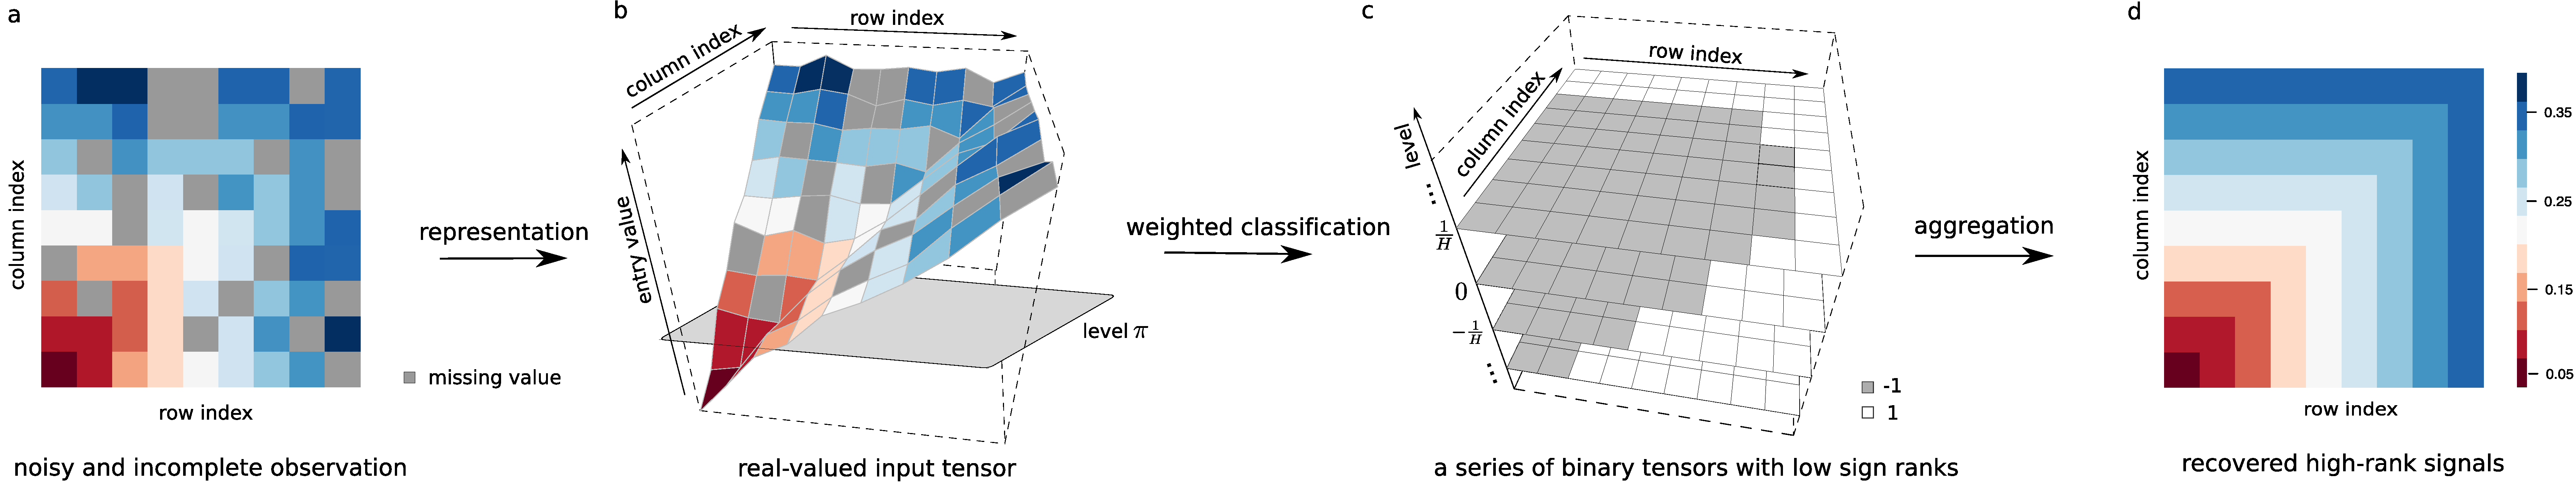
\includegraphics[width=1\textwidth]{image_new2.pdf}}
\caption{Illustration of our proposed method. For visualization purpose, we plot an order-2 tensor (a.k.a. matrix) in the figure; similar procedure applies to higher-order tensors. (a): input tensor $\tY_\Omega$ with noisy and incomplete entries. (b) and (c): our method uses weighted classification to estimate sign tensors $\sign(\Theta-\pi)$ for a sequence of levels $\pi\in \{-1,\ldots,-{1\over H},0,{1\over H},\ldots,1\}$. (d) output tensor $\hat \Theta$ with denoised and imputed entries. The depicted example is based on Example 5, where the true signal matrix has full rank. }\label{fig:demo}
\end{figure*}

Our observation is an incomplete data tensor from~\eqref{eq:model}, denoted $\tY_\Omega$, where $\Omega\subset[d_1]\times\cdots\times[d_K]$ is the index set of observed entries. We consider a general model on $\Omega$ that allows both uniform and non-uniform samplings. Specifically, let $\Pi=\{\pi_\omega\}$ be an arbitrarily predefined probability distribution over the full index set with $\sum_{\omega\in[d_1\times \cdots \times d_K]}\pi_\omega=1$. We assume the entries $\omega$ in $\Omega$ are i.i.d.\ draws with replacement from the full index set using distribution $\Pi$. The sampling rule will be denoted as $\omega\sim \Pi$.

Our goal is to accurately estimate $\Theta$ from the incomplete, noisy observation $\tY_\Omega$. In particular, we focus on the following two problems:
\begin{itemize}[leftmargin=*]
\item Q1 [Nonparametric tensor estimation]. How to flexibly estimate $\Theta$ under a wide range of structures, including both low-rankness and high-rankness?
\item Q2 [Tensor completion]. How many observed tensor entries do we need to consistently estimate the signal $\Theta$?
\end{itemize}


\subsection{Inadequacies of common low-rank models}\label{sec:example}
The signal plus noise model~\eqref{eq:model} is common in tensor literature. Most existing methods perform estimation based on the low-rankness of $\Theta$~\cite{anandkumar2014tensor,montanari2018spectral,kadmon2018statistical,cai2019nonconvex}. While these methods have shown great success in low-rank recovery, little is explored when the underlying signal tensor is of high rank. Here we provide two examples to illustrate the limitation of classical low-rank models.

The first example reveals the sensitivity of tensor rank to order-preserving transformations. Let $\tZ \in \mathbb{R}^{30\times 30\times 30}$ be an order-3 tensor with $\text{rank}(\tZ)=3$. Suppose a monotonic transformation $f(z)=(1+\exp(-cz))^{-1}$ is applied to $\tZ$ entrywise, and we observe data from model~\eqref{eq:model} with the signal tensor $\Theta=f(\tZ)$. Figure~\ref{fig:example}(a) plots the numerical rank of $\Theta$ versus $c$. Note that a smaller $c$ implies an approximate linear transformation $f(z)\approx -cz$, whereas a larger $c$ implies a higher nonlinearity $z\mapsto \{0,1\}$. As we see, the rank increases rapidly with $c$, rending traditional low-rank tensor methods ineffective even in the presence of mild order-preserving nonlinearities. In applications of digital processing and genomics analysis, the tensor of interest often undergoes some unknown transformation prior to measurements. The sensitivity to transformation therefore makes the low-rank model less desirable in practice. 

The second example shows that the classical low-rankness may exclude important specially-structured tensors. Here we consider the signal tensor of the form $\Theta=\log(1+\tZ)$, where $\tZ$ is an order-3 tensor with entries $\tZ(i,j,k)={1\over d}\max(i,j,k)$ for $(i,j,k)\in[d]^3$. In this case neither $\Theta$ nor $\tZ$ is low-rank; indeed, both tensors have rank lower bounded by dimension $d$ as illustrated in Figure~\ref{fig:example}(b) (proofs in Appendix). The matrix analogy of this $\Theta$ was studied in~\citet{chan2014consistent} in the context of graphon analysis. However, classical low-rank models fail to address these types of structures. 
\begin{figure}[h]
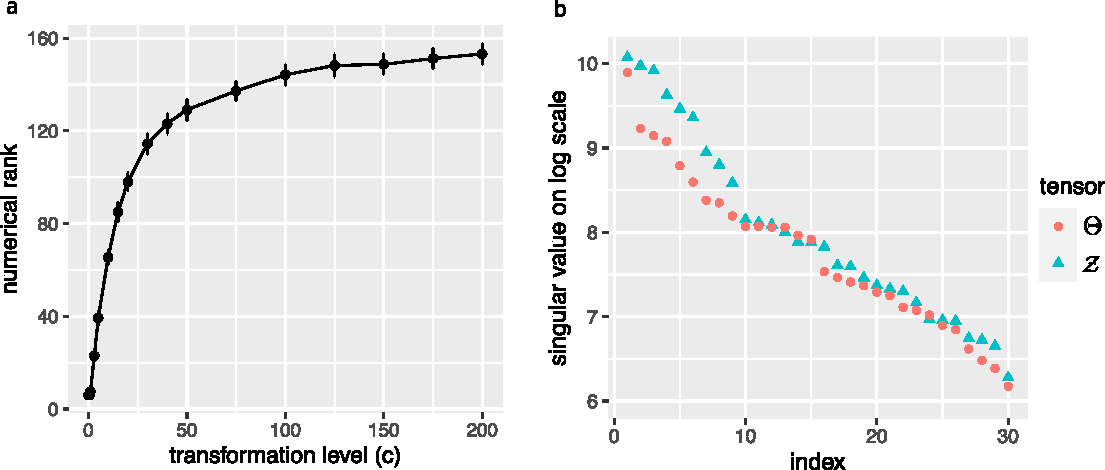
\includegraphics[width=.47\textwidth]{example_comb.pdf}
\caption{(a) Numerical rank of $\Theta=f(\tZ)$ versus $c$ in Example 1. Here, the numerical rank is computed as the minimal rank for which the relative least-squares error is below 0.1, and $\tZ$ is a rank-3 tensor with i.i.d.\ $N(0,1)$ entries in the (unnormalized) singular vectors. Reported ranks are averaged across 10 replicates of $\tZ$, with standard errors given in error bars. (b) Top $d=30$ tensor singular values in Example 2. Numerical values in both figures are obtained by running CP decomposition with random initialization.}\label{fig:example}
\end{figure}
In the above and many other examples, the signal tensors $\Theta$ exhibit high rank in spite of the special structures they admit. These structures are hardly detectable using classical low-rank models. New methods that allow flexible tensor modeling have yet to be developed. 

\subsection{Overview of our proposal}
Before describing our main results, we provide the intuition behind our method. In the earlier two examples, the high-rankness in the signal $\Theta$ makes the efficient estimation challenging. However, if we examine the sign of the $\pi$-shifted signal, $\sign(\Theta-\pi)$, for an arbitrary $\pi$ in the range of observations, then these sign tensors exhibit easily detectable low-rankness. For instance, the signal tensor in example 1 has the same sign pattern as a rank-$4$ tensor, since $\sign(\Theta-\pi)=\sign(\tZ-f^{-1}(\pi))$. The signal tensor in example 2 has the same sign pattern as a rank-2 tensor, since $\sign(\Theta-\pi)=\sign(\max(i,j,k)-d(e^{\pi}-1))$.

The above observation suggests a general framework to analyze both low- and high-rank signal tensors. Figure~\ref{fig:demo} illustrates the main crux of our method. We dichotomize the data tensor into a series of sign tensors, $\sign (\tY_\Omega-\pi)$, for $\pi\in \tH=\{-1,\ldots, {\scriptstyle -{1\over H}},0,{\scriptstyle {1\over H}},\ldots,1\}$, and then estimate the sign signals, $\sign(\Theta-\pi)$, by performing classification
\[
\hat \tZ_\pi=\argmin_{\text{low rank tensor $\tZ$}} L(\sign(\tZ),\ \sign (\tY_\Omega-\pi)).
\]
Here, $L(\cdot,\cdot)$ denotes a carefully-designed classification objective function which will be described in later sections. The final proposed tensor estimate is 
\[
\hat \Theta = {1\over 2H+1}\sum_{\pi \in \tH} \sign(\hat \tZ_\pi).
\]
Our approach is built on the nonparametric sign representation of signal tensors, and the estimate $\hat \Theta$ is essentially estimated from dichotomized tensor series $\{\sign(\tY_\Omega-\pi)\colon \pi \in \tH\}$. Surprisingly, we show that proper analysis based on dichotomized data not only preserves all information in the original signals, but also brings benefits of accuracy and flexibility over classical low-rank models. The method enjoys both statistical effectiveness and computational efficiency. 


\section{Sign representable tensors}\label{sec:representation}
In this section, we develop sign representable tensor models. The algebraic and statistical characterization of sign tensor series provides the accuracy guarantee for our method. 

\subsection{Sign-rank and sign tensor series}\label{sec:sign-rank}
Let $\Theta$ be a continuous-valued tensor, and $\sign (\Theta)$ be the corresponding sign patten. The sign pattern induces an equivalence relationship between tensors. Two tensors are called sign equivalent, denoted $\simeq$, if they share the same sign patterns. 

\begin{defn}[Sign-rank]
The sign-rank of a tensor $\Theta\in\mathbb{R}^{d_1\times \cdots \times d_L}$ is the minimal rank among all tensors that share the same sign patterns as $\Theta$; i.e.,
\[
\srank(\Theta) = \min \{\rank(\Theta')\colon  \Theta'\simeq \Theta,\ \Theta'\in\mathbb{R}^{d_1\times \cdots \times d_K}\}.
\]
\end{defn}
The sign-rank is also called \emph{support rank}~\cite{cohn2013fast}, \emph{minimal rank}~\cite{alon2016sign}, and \emph{nondeterministic rank}~\cite{de2003nondeterministic} in the filed of combinatorics and information theory. Earlier work defines sign-rank for binary tensors/matrices only; we extend the notion to continuous-valued tensors. Note that the sign-rank concerns only the sign pattern but discards the magnitudes information of $\Theta$. In particular, $\srank(\Theta)=\srank(\sign \Theta)$. 

Like most tensor problems~\cite{hillar2013most}, determining the sign-rank for a general tensor is NP hard~\cite{alon2016sign}. Fortunately, tensors arisen in application often possess special structures that facilitate analysis. We show that the family of low sign-rank tensors is strictly broader than usual low-rank tensors. This is because sign-rank is upper bounded by the usual rank. More generally, 
\begin{cor}[Upper bounds of sign-rank]~\label{cor:monotonic} For any monotonic function $g\colon \mathbb{R}\to \mathbb{R}$ with $g(0)=0$, 
\[
\textup{srank}(\Theta)\leq\rank(g(\Theta)).
\]
\end{cor}
Conversely, the sign-rank can be dramatically smaller than the usual rank, as we have shown in Section~\ref{sec:example}.
\begin{prop}[Broadness]\label{prop:extention}For every order $K\geq 2$ and dimension $d$, there exist order-$K$ $(d,\ldots,d)$-dimensional tensors $\Theta$ such that $\rank(\Theta)=d$ and $\srank(\Theta)=2$.
\end{prop}
We provide several common examples in Appendix where the tensor rank grows with dimension $d$ but the sign-rank remains a constant. The results highlight the advantages of using sign-rank in the high-dimensional tensor analysis. Corollary~\ref{cor:monotonic} and Proposition~\ref{prop:extention} together demonstrate the strict broadness of low sign-rank tensor family over the usual low-rank tensor family. 

We are now ready to introduce a family of tensors, which we coin as ``sign representable tensors'', as the signal tensors in model~\eqref{eq:model}. 
Without loss of generality, assume tensor entries are bounded by $A=1$. 
\begin{defn}[Sign representable tensors] 
Fix a level $\pi\in[-1,1]$. A tensor $\Theta$ is called $(r,\pi)$-sign representable, if the tensor $(\Theta-\pi)$ has sign-rank bounded by $r$. A tensor $\Theta$ is called $r$-sign (globally) representable, if $\Theta$ is $(r,\pi)$-sign representable for all $\pi\in[-1,1]$. The collection $\{\sign(\Theta-\pi)\colon \pi \in[-1,1]\}$ is called the sign tensor series. 
We use $\caliP(r)=\{\Theta\colon \srank(\Theta-\pi)\leq r \text{ for all }\pi\in[-1,1]\}$ to denote the $r$-sign representable tensor family.
\end{defn}
We show that the $r$-sign representable tensor family is a general model that incorporates most existing tensor models, including low-rank tensors, single index models, GLM models, and certain hypergraphon models. 

\begin{example}[CP/Tucker low-rank models] The CP and Tucker low-rank models are the two most popular tensor models~\cite{anandkumar2014tensor,montanari2018spectral,kadmon2018statistical,cai2019nonconvex}. Let $\Theta$ be a low-rank tensor with CP rank $r$. Then $\Theta$ belongs to the $r$-sign representable family, i.e., $\Theta\in\caliP(r)$. Similarly, Tucker low-rank tensors $\Theta\in\caliP(r)$, where $r=\prod_kr_k$ with $r_k$ being the $k$-th mode Tucker rank of $\Theta$.  
\end{example} 

\begin{example}[Generalized linear models (GLMs)] Let $\tY$ be a binary tensor from a tensor logistic model~\cite{wang2018learning} with mean $\Theta=\mathbb{E}(\tY)=\text{logit}(\tZ)$, where $\tZ$ is a latent low-rank tensor. Then, $\Theta$ is a special (parametric) case of sign representable tensors. Same conclusion holds for general exponential-family tensors with (known) distribution-specific link functions~\cite{hong2020generalized}.
\end{example}

\begin{example}[Single index models (SIMs)] Single index model is a flexible semiparametric model initially proposed in economics~\cite{robinson1988root} and has recently been popular in high-dimensional statistics~\cite{balabdaoui2019least,ganti2017learning,alquier2013sparse}. We here extend the model to high-dimensional tensors $\Theta$. The SIM assumes the existence of a (unknown) monotonic function $g\colon \mathbb{R}\to \mathbb{R}$ such that $g(\Theta)$ has rank $r$. We see that $\Theta$ belongs to the sign representable family; i.e., $\Theta\in \caliP(r+1)$. 
\end{example}

\begin{example}[Tensor block models (TBMs)] Tensor block model~\cite{wang2019multiway,chi2020provable} assumes a checkerbord structure among tensor entries under marginal index permutation. The signal tensor $\Theta$ takes at most $r$ distinct values, where $r$ is the total number of multiway blocks. Our model incorporates TBM because $\Theta \in \caliP(r)$. 
\end{example}

\begin{example}[Min/Max hypergraphon] Graphon is a popular nonparametric model for networks~\cite{chan2014consistent,xu2018rates}, and we have extended the model for tensors in Section~\ref{sec:example}. Here we revisit the model for generality. Let $\Theta$ be an order-$K$ tensor generated from the hypergraphon $\Theta(i_1,\ldots,i_K)=\log(1+\max_kx^{(k)}_{i_k})$, where $x^{(k)}_{i_k}\sim \text{Unif}[0,1]$ i.i.d.\ for all $i_k\in[d_k]$ and $k\in[K]$. Every sign tensor $\sign(\Theta-\pi)$ in the series of $\pi\in[0,\ \log 2]$ is a block tensor with at most two blocks, so $\Theta \in \caliP(2)$. 

More generally, let $g(\cdot)$ be a continuous univariate function with at most $r\geq 1$ real-valued roots in the equation $g(z)=\pi$; this property holds, e.g., when $g(z)$ is a polynomial of degree $r$. Then, the tensor $\Theta$ generated from $\Theta(i_1,\ldots,i_K)=g(\max_kx^{(k)}_{i_k})$ belongs to $\caliP(r+1)$. Same conclusion applies if the maximum is replaced by minimum.
\end{example}

\subsection{Statistical characterization of sign tensors via weighted classification}

Accurate estimation of a sign representable tensor crucially depends on the behavior of sign tensor series $\sign(\Theta-\pi)$. In this section, we show that weighted classification completely characterizes the sign tensors. The results bridge the algebraic and statistical properties of sign representable tensors, thereby providing the theoretical guarantee for our nonparametric algorithm (Figure~\ref{fig:demo}).
 
For a given $\pi \in [-1,1]$, define a $\pi$-shifted data tensor $\bar \tY_\Omega$ with entries $\bar \tY(\omega) = (\tY(\omega)-\pi)$ for all $\omega\in \Omega$. We propose a weighted classification objective
\begin{equation}\label{eq:sample}
L(\tZ, \bar \tY_\Omega)= {1\over |\Omega|}\sum_{\omega \in \Omega}\KeepStyleUnderBrace{|\bar \tY(\omega)|}_{\text{entry-specific weight}} \times \KeepStyleUnderBrace{| \sign \tZ(\omega)-\sign \bar \tY(\omega)|}_{\text{classification loss}},
\end{equation}
where $\tZ\in\mathbb{R}^{d_1\times \cdots \times d_K}$ is the decision variable to be optimized, $|\bar \tY(\omega)|$ is the entry-specific weight equal to the distance from the tensor entry to the target level $\pi$. The objective reduces to usual classification loss in the special case when the data tensor is binary and the target level $\pi=0$.

Our proposed entry-specific weight is important for characterizing $\sign(\Theta-\pi)$, as we show now. Define the weighted classification risk 
\begin{equation}\label{eq:population}
\textup{Risk}(\tZ)=\mathbb{E}_{\tY_\Omega}L(\tZ,\bar\tY_\Omega),
\end{equation}
where the expectation is taken with respect to $\tY_\Omega$ under model~\eqref{eq:model} and the sampling distribution $\omega\sim\Pi$. Note that the form of $\textup{Risk}(\cdot)$ implicitly depends on $\pi$; we suppress $\pi$ when no confusion arises. 
\begin{prop}[Global optimum of weighted risk]\label{prop:global}
Suppose the data $\tY_\Omega$ is generated from model~\eqref{eq:model} with $\Theta \in \caliP(r)$. Then, for all $\bar \Theta$ that are sign equivalent to $\sign(\Theta-\pi)$, 
\begin{align}\label{eq:optimal}
\textup{Risk}(\bar \Theta )&=\inf\{\textup{Risk}(\tZ)\colon \tZ\in\mathbb{R}^{d_1\times \cdots \times d_K}\},\notag \\
&=\inf\{\textup{Risk}(\tZ)\colon \textup{rank} \tZ\leq r\}.
\end{align}
\end{prop}
The results shows that the sign tensor $\sign(\Theta-\pi)$ optimizes the weighted classification risk. This fact suggests a practical procedure to estimate $\sign(\Theta-\pi)$ via optimizing the empirical risk $L(\tZ,\bar \tY_\Omega)$. The entry-specific weight incorporates the magnitude information in the classification, where entries far away from the target level are penalized more heavily in the objective. 

In order to establish the recovery guarantee, we address the uniqueness of the optimizer (up to sign equivalence) for $\risk(\cdot)$. Essentially, this is a converse problem of Proposition~\ref{prop:global} asking whether optimizing $\risk(\cdot)$ is sufficient for recovering $\sign(\Theta-\pi)$. The local behavior of $\Theta$ around $\pi$ turn out to play a key role in the accuracy guarantee. 

Some additional notation is needed. %Recall that $\omega\sim \Pi$ denotes the sampling distribution over tensor indices. 
We use $\tN=\{\pi\colon$  $\mathbb{P}_{\omega\sim \Pi}(\Theta(\omega)=\pi)\neq 0\}$ to denote the set of mass points of $\Theta$ under $\Pi$. Assume there exists a constant $C>0$, independent of tensor dimension, such that $|\tN|\leq C$. Note that both $\Pi$ and $\Theta$ implicitly depend on the tensor dimension. Our assumptions are imposed to $\Pi=\Pi(d)$ and $\Theta=\Theta(d)$ in the high-dimensional regime uniformly as $d:=\min_kd_k\to\infty$. 

%Unless otherwise stated, all relevant assumptions should be interpreted as uniform conditions for all large $d$. 

\begin{assumption}[$\alpha$-smoothness]\label{ass:margin} 
Fix $\pi\notin \tN$. Assume there exist constants $\alpha=\alpha(\pi)\geq 0, c=c(\pi) >0$, independent of tensor dimension, such that, 
\begin{equation}\label{eq:smooth}
\sup_{0\leq t<\rho(\pi, \tN)}{\mathbb{P}_{\omega \sim \Pi}(\omega \colon |\Theta (\omega)-\pi|\leq t )\over t^\alpha} \leq c,
\end{equation}
where $\rho(\pi,\tN):=\min_{\pi'\in \tN}|\pi-\pi'|$ denotes the distance from $\pi$ to the nearest point in $\tN$. The largest possible $\alpha=\alpha(\pi)$ is called the smoothness index at level $\pi$. We make the convention that $\alpha= \infty$ if the set $\{\omega\colon |\Theta(\omega)-\pi|\leq t\}$ has zero measure, implying few entries of $\Theta$ around the level $\pi$. We call the tensor $\Theta$ is $\alpha$-globally smooth, if~\eqref{eq:smooth} holds with a global constant $c>0$ for all $\pi\in[-1,1]$ except for a finite number of levels. 
\end{assumption}

The smoothness index $\alpha$ quantifies the intrinsic hardness of recovering $\sign(\Theta-\pi)$ from $\risk(\cdot)$. The recovery is more difficult at levels where the point mass concentrates (small $\alpha$). The value of $\alpha$ is determined by the marginal density of $\Theta(\omega)$ and the sampling distribution $\omega\sim \Pi$. A higher value of $\alpha>1$ corresponds a plateau-type zero density of $\Theta(\omega)$ around $\pi$, whereas a lower value of $\alpha<1$ indicates the nonexistence (infinite) density at level $\pi$. A typical case is $\alpha=1$ when $\Theta(\omega)$ has positive density bounded away from zero in the vicinity of $\pi$. 

{\color{red}Conjecture: If the global smoothness index $\alpha<1$, then $\tN\geq 1$. }


We now reach the main theorem in this section. For two tensors $\Theta_1,\Theta_2$, define the mean absolute error (MAE)
\[
\text{MAE}(\Theta_1, \Theta_2)\stackrel{\text{def}}{=}\mathbb{E}_{\omega\sim \Pi}\onenormSize{}{\Theta_1-\Theta_2}.
\]
\begin{thm}[Identifiability] Under Assumption~\ref{ass:margin}, for tensors $\bar \Theta \simeq \sign(\Theta-\pi)$ and all tensors $\tZ\in\mathbb{R}^{d_1\times \cdots \times d_K}$,
\[
\textup{MAE}(\sign \tZ, \sign \bar \Theta) \leq C(\pi)\left[\textup{Risk}(\tZ)-\textup{Risk}( \bar \Theta)\right]^{\alpha/(\alpha+1)},
\]
where $C(\pi)>0$ is independent of $\tZ$. 
\end{thm}
The result immediately suggests the uniqueness of the optimizer for $\text{Risk}(\cdot)$ up to a zero-measure set under $\Pi$, as long as $\alpha\neq 0$. Furthermore, the bound establishes the stability of recovering sign tensors $\sign (\Theta-\pi)$ from optimizing the population risk~\eqref{eq:population}. We find that a higher value of $\alpha$ implies more stable recovery. Similar results hold for the optimization problem with the empirical risk~\eqref{eq:sample} (Section~\ref{sec:estimation}). 

We conclude this section by relating Assumption~\ref{ass:margin} to the examples described in Section~\ref{sec:sign-rank}. 
We see that the tensor block model is $\infty$-globally smooth. This is because there are finitely many elements in $\tN$, i.e, the set of distinct block means in $\Theta$. Furthermore, we have $\alpha= \infty$ for all $\pi \notin \tN$, since the numerator in~\eqref{eq:smooth} is zero for all such $\pi$. The min/max hypergaphon with a $r$-degree polynomial function is $1$-globally smooth, because $\alpha=1$ for all $\pi$ in the function range except at most $(r-1)$ many (stationary) levels. 




\section{Nonparametric tensor completion via sign series}\label{sec:estimation}
In this section, we establish the statistical error bound for our nonparametric tensor method (Figure~\ref{fig:demo}). 

\subsection{Estimation error and sample complexity}
We cast the tensor completion problem into a series of weighted classifications, and propose the estimator
\begin{equation}\label{eq:est}
\hat \Theta = {1\over 2H+1}\sum_{\pi \in \tH}\sign{\hat \tZ_\pi},
\end{equation}
where $\hat \tZ_\pi\in\mathbb{R}^{d_1\times \dots\times d_K}$ is the estimated classifier at a series of levels $\pi \in \tH=\{-1,\ldots,-{1\over H}, 0, {1\over H},\ldots,1\}$,
\begin{equation}\label{eq:estimate}
\hat \tZ_\pi = \argmin_{\tZ\colon \text{rank}(\tZ)\leq r, \ \FnormSize{}{\tZ}\leq 1} L(\tZ, \sign(\tY_\Omega-\pi)).
\end{equation}
Here $L(\cdot,\cdot)$ denotes the weighted classification objective~\eqref{eq:sample}, and we have plugged in the $\pi$-shifted data tensor in the expression. The rank constraint on $\tZ$ is based on Proposition~\ref{prop:global}, and the Frobenius-norm constraint is a technical condition to simplify the analysis; the constraint does not alter the solution because $L(\tZ,\cdot)=L(\sign \tZ,\cdot)$ 

The next theorem establish the statistical convergence for the estimated sign tensor series~\eqref{eq:estimate}. For simplicity, we assume $d_1=\ldots=d_K=d$.

 \begin{thm}[Estimation of sign series]\label{thm:classification} Suppose $\Theta\in\caliP(r)$ and Assumption~\ref{ass:margin} holds at all level $\pi\notin \tN$ with smoothness index $\alpha\in[0,1]$. Then, for every such $\pi$, with very high probability over $\tY_\Omega$, 
\[
\textup{MAE}(\sign \hat \tZ_\pi, \sign(\Theta-\pi)) \lesssim \left({d r \over |\Omega|}\right)^{\alpha/(\alpha+2)}+{1\over \rho^2(\pi, \tN)} {dr \over |\Omega|}.
\]
\end{thm}
Theorem~\ref{thm:classification} provides the error bound for the estimated sign tensor series. The results shows that our sign estimator achieves consistent recovery using as few as $\tilde O(dr)$ noisy observations. Furthermore, our sign tensor estimation reaches a fast rate $d^{-(K-1)}$ when $\alpha=\infty$. The convergence rate becomes favorable as the order of data tensor increases. 

Using the connection between sign representable tensors and sign series, we obtain the main results on our nonparametric tensor estimation. 
\begin{thm}[Tensor estimation error]\label{thm:estimation} Consider the same condition of Theorem~\ref{thm:classification} and the nonparametric estimate $\hat \Theta$ in~\eqref{eq:est}. With very high probability over $\tY_\Omega$,
\[
\textup{MAE}(\hat \Theta, \Theta)\lesssim \left({d r \over |\Omega|}\right)^{\alpha/(\alpha+2)}+{1\over H}+H{d r \over |\Omega|}.
\]
Setting $H\asymp \left( |\Omega|\over rd\right)^{1/2}$ gives the estimation error bound
\[
\textup{MAE}(\hat \Theta, \Theta)\lesssim \left(dr \over|\Omega|\right)^{{\alpha \over \alpha+2} \vee {1\over 2}}.
\]
\end{thm}
Theorem~\ref{thm:estimation} demonstrates the fast convergence rate of our nonparamatric tensor estimation. Our results reveal three sources of errors: the estimation error inherited from sign estimation, the bias and the variance from sign series representations. The resolution parameter $H$ controls the bias-variance tradeoff.


Take-away: consistent is achieved whenever $|\Omega|/dr\to\infty$. Furthermore, with full observation $|\Omega|=d^K$, 
\[
\textup{MAE}(\hat \Theta, \Theta)\leq \left(r\over d^{(K-1)}\right)^{{\alpha \over \alpha+2} \vee {1\over 2}}.
\]
no faster than $d^{-(K-1)/2}$. Assuming MAE $\sim$ RMSE, the same (minimax) rate as in my NIPS paper. 

\begin{cor}[Sample complexity for completion] With very high probability 
\[
\textup{MAE}(\hat \Theta, \Theta)\to 0, \quad \text{as}\quad {|\Omega|\over dr}\to \infty.
\]
\end{cor}


\begin{example}[Tensor block model]
Consider tensor block model. $\alpha=\infty$. Earlier results show the estimation error
\[
\textup{MAE}(\hat \Theta, \Theta)\leq \sqrt{r\log d \over |\Omega|}.
\]
Compare to existing literature. Assuming MAE $\sim$ RMSE, the same (minimax) rate as in my NIPS paper. 
 
\end{example}
\begin{example}[Single index and Min/Max hypographon tensor model]
$\tO(d^{-(K-1)/3})$. Slightly worst than~\citet{ganti2015matrix}.
\end{example}

\subsection{Numerical implementation}
In practice, the optimization~\eqref{eq:estimate} can be impelmented using an efficient divide-and-conquer fashion. The estimation of sign tensors is parallelable for the series $\pi \in \tH$ through parallel implementation. 

For each $\pi\in\tH$, an alternating optimization algorithm is developed to solve~\eqref{eq:estimate}. Following the common practice in classification, we replace the binary loss $\ell(z,y)=|\sign z - \sign y|$ with a more manageable surrogate loss $F(m)$ as a function of margin $m\stackrel{\text{def}}{=}z\sign(y)$. Examples of large-margin loss are hinge loss $F(m) = (1-m)_+$ for support vector machines, logistic loss $F(m) =\log(1+e^{-m})$ for important vector machines, and nonconvex $\psi$-loss $F(m)=2\min(1,(1-m)_+)$ with $m_{+}=\max(m,0)$. We implement the hinge loss and logistic loss for illustration, although our framework is applicable to general large-margin losses~\citep{bartlett2006convexity}. 

The rank constraint is implemented by using the rank decomposition as in~\eqref{eq:CP} and optimizing one factor of $\tZ$ at a time while holding others fixed. Each suboptimization reduces to a classical weighted classification with a $(rd_k)$-dimensional decision variable. As common in tensor optimization, we run the algorithm from multiple initializations for locate a final estimate with the lowest objective value. The full procedure is described in Algorithm 1.

\begin{figure*}[h]
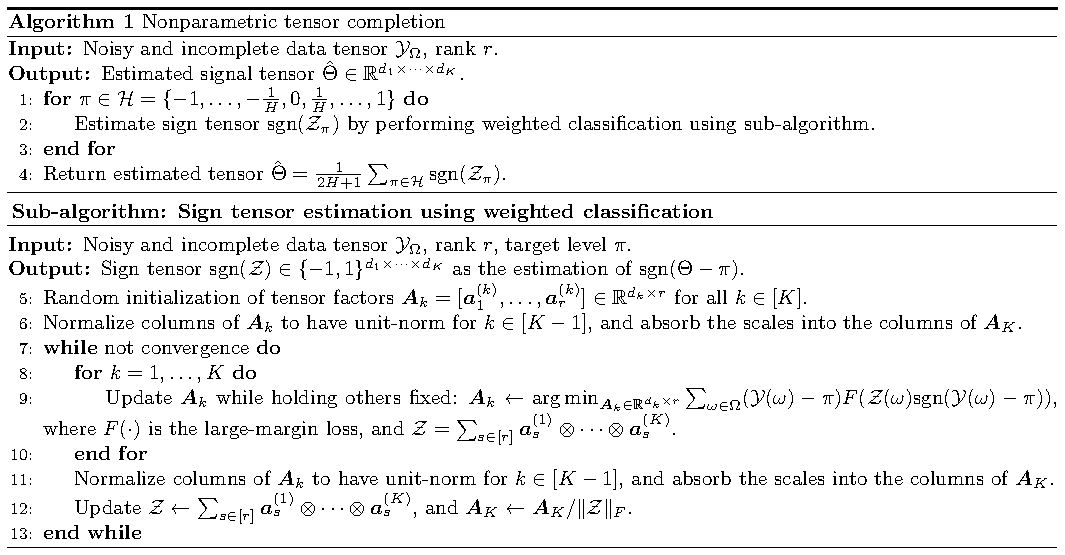
\includegraphics[width=\textwidth]{algorithm.pdf}
\end{figure*}



\clearpage
\begingroup
\let\clearpage\relax 
\onecolumn 
%\begin{prop}
%Let $\Theta=\sum_{r=1}^d\me_r^{\otimes 3}$ be the identity tensor, where $\me_r=(0,\ldots,0,1,0,\ldots,0)^T$ is the $r$-th canonical basis in $\mathbb{R}^d$. Then $\rank(\Theta)=d$ and $\srank(\Theta)=2$. 
%\end{prop}
\begin{example}[Addition examples that satisfying Proposition~\ref{prop:extention}]
We provide a tensor example with $\rank(\Theta)=d$ but $\srank(\Theta)=3$. Define $\Theta=\sum_{r=1}^d \me^{\otimes 2}_r\otimes \mathbf{1}^{\otimes (K-2)}_d$, where $\me_r=(0,\ldots,0,1,0,\ldots,0)^T$ is the $r$-th canonical basis in $\mathbb{R}^d$, and $\mathbf{1}_d\in\mathbb{R}^d$ is a vector with all entries 1. Based on the definition of $\Theta$, we have
\[
\rank(\Theta)=\rank(\mI),\quad \srank(\Theta)=\srank(\mI),
\]
where $\mI\in\mathbb{R}^{d\times d}$ is the identity matrix. Therefore, it suffices to show that $\srank(\mI)=3$. We now construct a rank-2 matrix $\mA$ such that $\sign(\mA-1/2)=\sign(\mI)$. Define
\[
\mA=\begin{bmatrix}
1 & -{1\over 2}\times 1\\
2^{-1}& -{1\over 2}\times 4^{-1}\\
\vdots&\vdots\\
2^{-d+1}& -{1\over 2}\times 4^{-d+1}
\end{bmatrix}
\begin{bmatrix}
1&2&\cdots&2^{d-1}\\
1&4&\cdots& 4^{d-1}
\end{bmatrix}.
\]
It is easy to verify that $\mA(i,j)={1\over 2}$ if $i=j$, and $\mA(i,j)<{1\over 2}$ otherwise. Therefore, $\sign(\mA-1/2)=\mI$. 
\end{example}
\begin{proof}[Proof of Proposition~\ref{prop:global}]
Based on the definition, the function $\risk(\cdot)$ relies only on the sign pattern of the tensor. Therefore, without loss of generality, we assume both tensors $\bar \Theta, \tZ \in\{-1,1\}^{d_1\times \cdots \times d_K}$ are binary tensors. 
We evaluate the excess risk 
\begin{equation}\label{eq:risk}
\risk(\tZ)- \risk(\bar \Theta) = \mathbb{E}_{\omega\sim \Pi}\KeepStyleUnderBrace{\mathbb{E}_{\tY(\omega)}\left\{|\tY(\omega)-\pi|\left[\left|\tZ(\omega)-\sign(\bar \tY(\omega)) \right|-\left|\bar\Theta(\omega)-\sign(\bar \tY(\omega))\right|\right]\right\}}_{=:I(\omega)}.
\end{equation}
Denote $y=\tY(\omega)$, $z=\tZ(\omega)$, $\bar \theta=\bar\Theta(\omega)$, and $\theta=\Theta(\omega)$. It follows from the expression of $I(\omega)$ that
\begin{align}\label{eq:I}
I(\omega)&= \mathbb{E}_{y}\left[ (y-\pi)(\bar \theta-z)\mathds{1}(y\geq \pi)+(\pi-y)(z-\bar \theta)\mathds{1}(y< \pi)\right]\\
&= \mathbb{E}_{y}\left[(\bar \theta-z) (y-\pi)\right]\\
&=  \left[\sign(\theta-\pi)-z\right]\left(\theta-\pi\right)\\
&= |\sign(\theta-\pi)-z||\theta-\pi|\geq 0
\end{align}
where the third line uses the fact $\mathbb{E}y=\theta$ and $\bar \theta=\sign(\theta-\pi)$, and the last line uses the assumption $z \in\{-1,1\}$. In particular, the equality is attained when $z=\sign(\theta-\pi)$ or $\theta=\pi$. Combining~\eqref{eq:I} with~\eqref{eq:risk}, we conclude 
\[
\risk(\tZ)- \risk(\bar \Theta) = \mathbb{E}_{\omega\sim \Pi} |\sign(\Theta(\omega)-\pi)-\tZ(\omega)||\Theta(\omega)-\pi|\geq 0,
\]
for all $\tZ\in\{-1,1\}^{d_1\times \cdots \times d_K}$. Therefore,
\[
\risk(\bar \Theta)=\min\{\risk(\tZ)\colon \tZ\in \mathbb{R}^{d_1\times \cdots \times d_K}\} \leq \min\{\risk(\tZ)\colon \rank(\tZ)\leq r\}.
\]
Because $\srank(\bar \Theta)\leq r$ by assumption, the last inequality becomes equality. The proof is complete. 
\end{proof}


\begin{proof}
We verify two conditions. 
\begin{enumerate}
\item Approximation error. For $\tZ$ with $\text{rank}(\tZ)\leq r$, we have $\textup{Risk}(\tZ)-\textup{Risk}(\bar \Theta)=0$ for all $d$.  
\item Variance-to-mean relationship
\[
\text{Var}_{\tY, \Omega}[L(\tZ,\bar \tY_\pi)-L(\bar \Theta, \tY_\pi)]\leq [\textup{Risk}(\tZ)-\textup{Risk}(\bar \Theta)]^{\alpha/(1+\alpha)}+{1\over \rho(\pi, \tN)}[\textup{Risk}(\tZ)-\textup{Risk}(\bar \Theta)].
\]
Apply Lemma~\ref{lem:tensor} to the above condition, we obtain
\[
\textup{Risk}(\tZ)-\textup{Risk}(\bar \Theta)\leq t_n^{(\alpha+1)/(\alpha+2)}+{1\over \rho(\pi, \tN)}t_n, \quad \text{where }t_n={Krd\over n}.
\]
\end{enumerate}
\end{proof}

\begin{lem}\label{lem:tensor}

Because the classification rate is scale-free; $\text{Risk}(\tZ)=\text{Risk}(c\tZ)$ for every $c>0$. Therefore, without loss of generality, we solve the estimate subject to $\FnormSize{}{\tZ}\leq 1$,
\[
\hat \tZ=\argmin_{\tZ\colon \textup{rank}(\tZ)\leq r, \FnormSize{}{\tZ}\leq 1}L(\tZ,\bar \tY_\pi).
\]
Write $|\Omega|=n$. We have
\[
\mathbb{P}[\textup{Risk}(\hat \tZ)-\textup{Risk}(\bar \Theta)\geq t_n]\leq {7\over 2}\exp(-Cnt_n).
\]
The rate of convergence $t_n>0$ is determined by the solution to the following inequality,
\[
{1\over t_n}\int^{\sqrt{t_n^\alpha+\rho^{-1}t_n}}_{t_n} \sqrt{\tH_{[\ ]}(\varepsilon,\ \tF,\ \vnormSize{}{\cdot}) }d\varepsilon \leq n^{1/2}, 
\]
where $\tF=\{\tZ\colon \textup{rank}(\tZ)\leq r, \ \FnormSize{}{\tZ}^2\leq 1\}$ and $\rho=\rho(\pi, \tN)$. By Lemma~\ref{lem:bracketing}, we obtain 
\[
t_n\asymp \left({Kdr\over n}\right)^{(\alpha+1)/(\alpha+2)} +{1\over \rho^2(\pi, \tN)} {Kdr\over n}.
\] 
Finally, we obtain
\[
\mathbb{P}[\textup{Risk}(\hat \tZ)-\textup{Risk}(\bar \Theta)\geq t_n]\leq {7\over 2}\exp(-Cd^{\alpha+1\over \alpha+2}n^{1\over \alpha+2}) \leq {7\over 2}\exp(-C\sqrt{d}),
\]
where $C=C(k,r)>0$ is a constant independent of $d$ and $n$.  
\end{lem}

\begin{lem}[Bracketing number for bounded low rank tensor]\label{lem:bracketing}
\[
\sqrt{\mathbb{E}_{\omega\sim \Pi}|\tZ_1(\omega)-\tZ_2(\omega)|^2} \leq \mnormSize{}{\tZ_1-\tZ_2} \leq \FnormSize{}{\tZ_1-\tZ_2}.
\]
Therefore
\[
\tH_{[\ ]}(2\varepsilon, \tF, \vnormSize{}{\cdot})\leq \tH(\varepsilon, \tF, \FnormSize{}{\cdot}) \leq C{(1+Kdr)\log {d\over \varepsilon}},
\]
where the covering number for low rank tensor is based on~\citet{mu2014square,9119759}.
\end{lem}
\endgroup


\bibliographystyle{chicago}

\bibliography{tensor_wang}

\appendix

\end{document}
